% begin module cycloid-def
\begin{frame}
\frametitle{The Cycloid}

\psset{xunit=0.8cm, yunit=0.8cm}
\begin{pspicture}(-1.499950, -0.5)(14.066321,5)
\psframe*[linecolor=white](-1.499950,-0.1)(14.066321,5)
\tiny

%circles generated by calculator commands:
%precision:=0.99995;f{}{{t}}:=plot2D(\sqrt{1-(x-t)^2}+1, t-precision, t+precision )+plot2D(-\sqrt{1-(x-t)^2}+1, t-precision, t+precision );f{}(0)+f{}(0.5\pi)+f{}(\pi)+f{}(1.5\pi)+f{}(2\pi)+f{}(2.5\pi)+f{}(3\pi)+f{}(3.5\pi)+f{}(4\pi)

\fcAxesStandard{-1.1}{-0.5}{13.566321}{2.3}

%calcululator commands: f{}{{t}}:=(DoubleValue (t\pi-sin (t\pi) ), 1-cos (\pi t));(f{}0, f{}0.5, f{}1, f{}1.5, f{}2, f{}2.5, f{}3, f{}3.5, f{}4)
%generate the following points:
%(0.000000, 0.000000), (0.570796, 1.000000), (3.141593, 2), (5.712389, 1.000000), (6.283185, 0.000000), (6.853982, 1.000000), (9.424778, 2.000000), (11.995574, 1.000000), (12.566371, 0.000000)

\uncover<1>{
%Function formula: (- x^{2}+1)^{1/2}+1
\psplot[linecolor=\fcColorTangent, plotpoints=1000]{-0.999990}{0.999990}{1.0000000 1.0000000 x 2.0000000 exp -1.0000000 mul add 0.5000000 exp add }
%Function formula: - (- x^{2}+1)^{1/2}+1
\psplot[linecolor=\fcColorTangent, plotpoints=1000]{-0.999990}{0.999990}{1.0000000 1.0000000 x 2.0000000 exp -1.0000000 mul add 0.5000000 exp -1.0000000 mul add }
\fcFullDot{0}{0}
\rput[bl](0.1, 0.1){$P$}
}

\uncover<2>{
%Function formula: (- (x-1/2 \pi)^{2}+1)^{1/2}+1
\psplot[linecolor=\fcColorTangent, plotpoints=1000]{0.570806}{2.570786}{1.0000000 1.0000000 3.141592654 -0.5000000 mul x add 2.0000000 exp -1.0000000 mul add 0.5000000 exp add }
%Function formula: - (- (x-1/2 \pi)^{2}+1)^{1/2}+1
\psplot[linecolor=\fcColorTangent, plotpoints=1000]{0.570806}{2.570786}{1.0000000 1.0000000 3.141592654 -0.5000000 mul x add 2.0000000 exp -1.0000000 mul add 0.5000000 exp -1.0000000 mul add }
\fcFullDot{0.570796}{1}
\rput[l](0.670796, 1.000000){$P$}
}

\uncover<3>{
%Function formula: (- (x- \pi)^{2}+1)^{1/2}+1
\psplot[linecolor=\fcColorTangent, plotpoints=1000]{2.141603}{4.141583}{1.0000000 1.0000000 3.141592654 -1.0000000 mul x add 2.0000000 exp -1.0000000 mul add 0.5000000 exp add }
%Function formula: - (- (x- \pi)^{2}+1)^{1/2}+1
\psplot[linecolor=\fcColorTangent, plotpoints=1000]{2.141603}{4.141583}{1.0000000 1.0000000 3.141592654 -1.0000000 mul x add 2.0000000 exp -1.0000000 mul add 0.5000000 exp -1.0000000 mul add }
\fcFullDot{3.141593}{2}
\rput[t](3.141593, 1.9){$P$}
}

\uncover<4>{
%Function formula: (- (x-3/2 \pi)^{2}+1)^{1/2}+1
\psplot[linecolor=\fcColorTangent, plotpoints=1000]{3.712399}{5.712379}{1.0000000 1.0000000 3.141592654 -1.5000000 mul x add 2.0000000 exp -1.0000000 mul add 0.5000000 exp add }
%Function formula: - (- (x-3/2 \pi)^{2}+1)^{1/2}+1
\psplot[linecolor=\fcColorTangent, plotpoints=1000]{3.712399}{5.712379}{1.0000000 1.0000000 3.141592654 -1.5000000 mul x add 2.0000000 exp -1.0000000 mul add 0.5000000 exp -1.0000000 mul add }
\fcFullDot{5.712389}{1}
\rput[r](5.612389, 1){$P$}
}

\uncover<5>{
%Function formula: - (- (x-2 \pi)^{2}+1)^{1/2}+1
\psplot[linecolor=\fcColorTangent, plotpoints=1000]{5.283195}{7.283175}{1.0000000 1.0000000 3.141592654 -2.0000000 mul x add 2.0000000 exp -1.0000000 mul add 0.5000000 exp -1.0000000 mul add }
%Function formula: (- (x-2 \pi)^{2}+1)^{1/2}+1
\psplot[linecolor=\fcColorTangent, plotpoints=1000]{5.283195}{7.283175}{1.0000000 1.0000000 3.141592654 -2.0000000 mul x add 2.0000000 exp -1.0000000 mul add 0.5000000 exp add }
\fcFullDot{6.283185}{0}
\rput[lb](6.283185, 0.1){$P$}
}

\uncover<6>{
%Function formula: (- (x-5/2 \pi)^{2}+1)^{1/2}+1
\psplot[linecolor=\fcColorTangent, plotpoints=1000]{6.853992}{8.853972}{1.0000000 1.0000000 3.141592654 -2.5000000 mul x add 2.0000000 exp -1.0000000 mul add 0.5000000 exp add }
%Function formula: - (- (x-5/2 \pi)^{2}+1)^{1/2}+1
\psplot[linecolor=\fcColorTangent, plotpoints=1000]{6.853992}{8.853972}{1.0000000 1.0000000 3.141592654 -2.5000000 mul x add 2.0000000 exp -1.0000000 mul add 0.5000000 exp -1.0000000 mul add }
\fcFullDot{6.853982}{1}
\rput[l](6.953982, 1.000000){$P$}
}

\uncover<7>{
%Function formula: (- (x-3 \pi)^{2}+1)^{1/2}+1
\psplot[linecolor=\fcColorTangent, plotpoints=1000]{8.424788}{10.424768}{1.0000000 1.0000000 3.141592654 -3.0000000 mul x add 2.0000000 exp -1.0000000 mul add 0.5000000 exp add }
%Function formula: - (- (x-3 \pi)^{2}+1)^{1/2}+1
\psplot[linecolor=\fcColorTangent, plotpoints=1000]{8.424788}{10.424768}{1.0000000 1.0000000 3.141592654 -3.0000000 mul x add 2.0000000 exp -1.0000000 mul add 0.5000000 exp -1.0000000 mul add }
\fcFullDot{9.424778}{2}
\rput[t](9.424778, 1.9){$P$}
}

\uncover<8>{
%Function formula: - (- (x-7/2 \pi)^{2}+1)^{1/2}+1
\psplot[linecolor=\fcColorTangent, plotpoints=1000]{9.995584}{11.995564}{1.0000000 1.0000000 3.141592654 -3.5000000 mul x add 2.0000000 exp -1.0000000 mul add 0.5000000 exp -1.0000000 mul add }
%Function formula: (- (x-7/2 \pi)^{2}+1)^{1/2}+1
\psplot[linecolor=\fcColorTangent, plotpoints=1000]{9.995584}{11.995564}{1.0000000 1.0000000 3.141592654 -3.5000000 mul x add 2.0000000 exp -1.0000000 mul add 0.5000000 exp add }
\fcFullDot{11.995574}{1}
\rput[r](11.895574, 1.000000){$P$}
}

\uncover<9>{
%Function formula: (- (x-4 \pi)^{2}+1)^{1/2}+1
\psplot[linecolor=\fcColorTangent, plotpoints=1000]{11.566381}{13.566361}{1.0000000 1.0000000 3.141592654 -4.0000000 mul x add 2.0000000 exp -1.0000000 mul add 0.5000000 exp add }
%Function formula: - (- (x-4 \pi)^{2}+1)^{1/2}+1
\psplot[linecolor=\fcColorTangent, plotpoints=1000]{11.566381}{13.566361}{1.0000000 1.0000000 3.141592654 -4.0000000 mul x add 2.0000000 exp -1.0000000 mul add 0.5000000 exp -1.0000000 mul add }
\fcFullDot{12.566371}{0}
\rput[lb](12.566371, 0.1){$P$}
}

%Calculator input:f{}{{p}}:=plotCurve(t+\cos(- t+3\pi/2), 1+\sin(3\pi/2- t),p, p+\pi/4)+ plotCurve(t+\cos(- t+3\pi/2), 1+\sin(3\pi/2- t), p+\pi/4, p+\pi/2); f{}0+f{}(0.5\pi)+ f{}(\pi)+f{}(1.5\pi)+f{}(2\pi)+f{}(2.5\pi)+f{}(3\pi)+f{}(3.5\pi)+f{}(4\pi)


\uncover<2->{
%Calculator input: plotCurve{}(\cos{}(- t+3/2 \pi)+t, \sin{}(- t+3/2 \pi)+1, 0, 1/4 \pi)
\parametricplot[linecolor=\fcColorGraph, arrows=->, plotpoints=1000]{0}{0.785398}{t 3.141592654 1.5000000 mul t -1.0000000 mul add 57.29578 mul cos add 1.0000000 3.141592654 1.5000000 mul t -1.0000000 mul add 57.29578 mul sin add }
%Calculator input: plotCurve{}(\cos{}(- t+3/2 \pi)+t, \sin{}(- t+3/2 \pi)+1, 1/4 \pi, 1/2 \pi)
\parametricplot[linecolor=\fcColorGraph, plotpoints=1000]{ 0.785398}{1.5708}{t 3.141592654 1.5000000 mul t -1.0000000 mul add 57.29578 mul cos add 1.0000000 3.141592654 1.5000000 mul t -1.0000000 mul add 57.29578 mul sin add }
}
\uncover<3->{
%Calculator input: plotCurve{}(\cos{}(- t+3/2 \pi)+t, \sin{}(- t+3/2 \pi)+1, 1/2 \pi, 3/4 \pi)
\parametricplot[linecolor=\fcColorGraph, arrows=->, plotpoints=1000]{1.5708}{2.35619}{t 3.141592654 1.5000000 mul t -1.0000000 mul add 57.29578 mul cos add 1.0000000 3.141592654 1.5000000 mul t -1.0000000 mul add 57.29578 mul sin add }
%Calculator input: plotCurve{}(\cos{}(- t+3/2 \pi)+t, \sin{}(- t+3/2 \pi)+1, 3/4 \pi, \pi)
\parametricplot[linecolor=\fcColorGraph, plotpoints=1000]{2.35619}{3.14159}{t 3.141592654 1.5000000 mul t -1.0000000 mul add 57.29578 mul cos add 1.0000000 3.141592654 1.5000000 mul t -1.0000000 mul add 57.29578 mul sin add }
}
\uncover<4->{
%Calculator input: plotCurve{}(\cos{}(- t+3/2 \pi)+t, \sin{}(- t+3/2 \pi)+1, \pi, 5/4 \pi)
\parametricplot[linecolor=\fcColorGraph, arrows=->, plotpoints=1000]{3.14159}{3.92699}{t 3.141592654 1.5000000 mul t -1.0000000 mul add 57.29578 mul cos add 1.0000000 3.141592654 1.5000000 mul t -1.0000000 mul add 57.29578 mul sin add }
%Calculator input: plotCurve{}(\cos{}(- t+3/2 \pi)+t, \sin{}(- t+3/2 \pi)+1, 5/4 \pi, 3/2 \pi)
\parametricplot[linecolor=\fcColorGraph, plotpoints=1000]{3.92699}{4.71239}{t 3.141592654 1.5000000 mul t -1.0000000 mul add 57.29578 mul cos add 1.0000000 3.141592654 1.5000000 mul t -1.0000000 mul add 57.29578 mul sin add }
}
\uncover<5->{
%Calculator input: plotCurve{}(\cos{}(- t+3/2 \pi)+t, \sin{}(- t+3/2 \pi)+1, 3/2 \pi, 7/4 \pi)
\parametricplot[linecolor=\fcColorGraph, arrows=->, plotpoints=1000]{4.71239}{5.49779}{t 3.141592654 1.5000000 mul t -1.0000000 mul add 57.29578 mul cos add 1.0000000 3.141592654 1.5000000 mul t -1.0000000 mul add 57.29578 mul sin add }
%Calculator input: plotCurve{}(\cos{}(- t+3/2 \pi)+t, \sin{}(- t+3/2 \pi)+1, 7/4 \pi, 2 \pi)
\parametricplot[linecolor=\fcColorGraph, plotpoints=1000]{5.49779}{6.28319}{t 3.141592654 1.5000000 mul t -1.0000000 mul add 57.29578 mul cos add 1.0000000 3.141592654 1.5000000 mul t -1.0000000 mul add 57.29578 mul sin add }
}
\uncover<6->{
%Calculator input: plotCurve{}(\cos{}(- t+3/2 \pi)+t, \sin{}(- t+3/2 \pi)+1, 2 \pi, 9/4 \pi)
\parametricplot[linecolor=\fcColorGraph, arrows=->, plotpoints=1000]{6.28319}{7.06858}{t 3.141592654 1.5000000 mul t -1.0000000 mul add 57.29578 mul cos add 1.0000000 3.141592654 1.5000000 mul t -1.0000000 mul add 57.29578 mul sin add }
%Calculator input: plotCurve{}(\cos{}(- t+3/2 \pi)+t, \sin{}(- t+3/2 \pi)+1, 9/4 \pi, 5/2 \pi)
\parametricplot[linecolor=\fcColorGraph, plotpoints=1000]{7.06858}{7.85398}{t 3.141592654 1.5000000 mul t -1.0000000 mul add 57.29578 mul cos add 1.0000000 3.141592654 1.5000000 mul t -1.0000000 mul add 57.29578 mul sin add }
}
\uncover<7->{
%Calculator input: plotCurve{}(\cos{}(- t+3/2 \pi)+t, \sin{}(- t+3/2 \pi)+1, 5/2 \pi, 11/4 \pi)
\parametricplot[linecolor=\fcColorGraph, arrows=->, plotpoints=1000]{7.85398}{8.63938}{t 3.141592654 1.5000000 mul t -1.0000000 mul add 57.29578 mul cos add 1.0000000 3.141592654 1.5000000 mul t -1.0000000 mul add 57.29578 mul sin add }
%Calculator input: plotCurve{}(\cos{}(- t+3/2 \pi)+t, \sin{}(- t+3/2 \pi)+1, 11/4 \pi, 3 \pi)
\parametricplot[linecolor=\fcColorGraph, plotpoints=1000]{8.63938}{9.42478}{t 3.141592654 1.5000000 mul t -1.0000000 mul add 57.29578 mul cos add 1.0000000 3.141592654 1.5000000 mul t -1.0000000 mul add 57.29578 mul sin add }
}
\uncover<8->{
%Calculator input: plotCurve{}(\cos{}(- t+3/2 \pi)+t, \sin{}(- t+3/2 \pi)+1, 3 \pi, 13/4 \pi)
\parametricplot[linecolor=\fcColorGraph, arrows=->, plotpoints=1000]{9.42478}{10.2102}{t 3.141592654 1.5000000 mul t -1.0000000 mul add 57.29578 mul cos add 1.0000000 3.141592654 1.5000000 mul t -1.0000000 mul add 57.29578 mul sin add }
%Calculator input: plotCurve{}(\cos{}(- t+3/2 \pi)+t, \sin{}(- t+3/2 \pi)+1, 13/4 \pi, 7/2 \pi)
\parametricplot[linecolor=\fcColorGraph, plotpoints=1000]{10.2102}{10.9956}{t 3.141592654 1.5000000 mul t -1.0000000 mul add 57.29578 mul cos add 1.0000000 3.141592654 1.5000000 mul t -1.0000000 mul add 57.29578 mul sin add }
}
\uncover<9->{
%Calculator input: plotCurve{}(\cos{}(- t+3/2 \pi)+t, \sin{}(- t+3/2 \pi)+1, 7/2 \pi, 15/4 \pi)
\parametricplot[linecolor=\fcColorGraph, arrows=->, plotpoints=1000]{10.9956}{11.781}{t 3.141592654 1.5000000 mul t -1.0000000 mul add 57.29578 mul cos add 1.0000000 3.141592654 1.5000000 mul t -1.0000000 mul add 57.29578 mul sin add }
%Calculator input: plotCurve{}(\cos{}(- t+3/2 \pi)+t, \sin{}(- t+3/2 \pi)+1, 15/4 \pi, 4 \pi)
\parametricplot[linecolor=\fcColorGraph, plotpoints=1000]{11.781}{12.5664}{t 3.141592654 1.5000000 mul t -1.0000000 mul add 57.29578 mul cos add 1.0000000 3.141592654 1.5000000 mul t -1.0000000 mul add 57.29578 mul sin add }
}
\uncover<10->{
%Calculator input: plotCurve{}(\cos{}(- t+3/2 \pi)+t, \sin{}(- t+3/2 \pi)+1, 4 \pi, 17/4 \pi)
\parametricplot[linecolor=\fcColorGraph, arrows=->, plotpoints=1000]{12.5664}{13.3518}{t 3.141592654 1.5000000 mul t -1.0000000 mul add 57.29578 mul cos add 1.0000000 3.141592654 1.5000000 mul t -1.0000000 mul add 57.29578 mul sin add }
%Calculator input: plotCurve{}(\cos{}(- t+3/2 \pi)+t, \sin{}(- t+3/2 \pi)+1, 17/4 \pi, 9/2 \pi)
\parametricplot[linecolor=\fcColorGraph, plotpoints=1000]{13.3518}{14.1372}{t 3.141592654 1.5000000 mul t -1.0000000 mul add 57.29578 mul cos add 1.0000000 3.141592654 1.5000000 mul t -1.0000000 mul add 57.29578 mul sin add }
}
\end{pspicture}

\begin{definition}[Cycloid]
The curve traced out by a point $P$ on the circumference of a circle as the circle rolls along a straight line is called a cycloid. \uncover<11>{}
\end{definition}

%\ \only<handout:0| 1>{%
%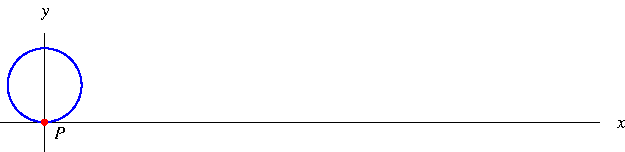
\includegraphics[width=12cm]{parametric-curves/pictures/11-01-cycloida.pdf}%
%}%
%\only<handout:0| 2>{%
%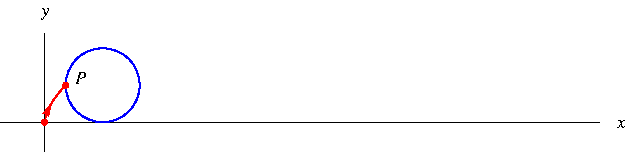
\includegraphics[width=12cm]{parametric-curves/pictures/11-01-cycloidb.pdf}%
%}%
%\only<handout:0| 3>{%
%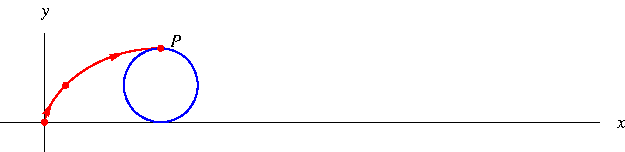
\includegraphics[width=12cm]{parametric-curves/pictures/11-01-cycloidc.pdf}%
%}%
%\only<handout:0| 4>{%
%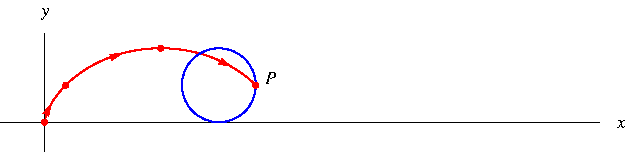
\includegraphics[width=12cm]{parametric-curves/pictures/11-01-cycloidd.pdf}%
%}%
%\only<handout:0| 5>{%
%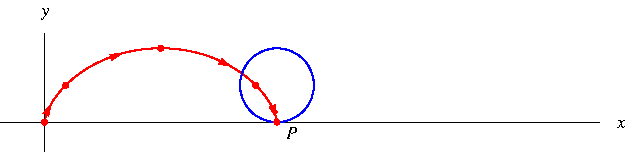
\includegraphics[width=12cm]{parametric-curves/pictures/11-01-cycloide.pdf}%
%}%
%\only<handout:0| 6>{%
%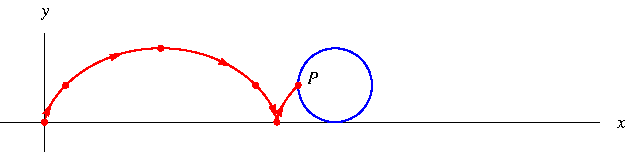
\includegraphics[width=12cm]{parametric-curves/pictures/11-01-cycloidf.pdf}%
%}%
%\only<handout:0| 7>{%
%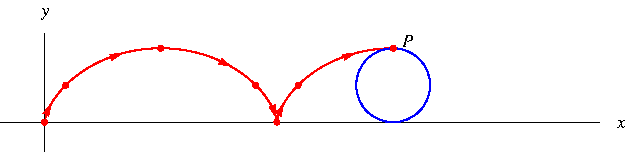
\includegraphics[width=12cm]{parametric-curves/pictures/11-01-cycloidg.pdf}%
%}%
%\only<8>{%
%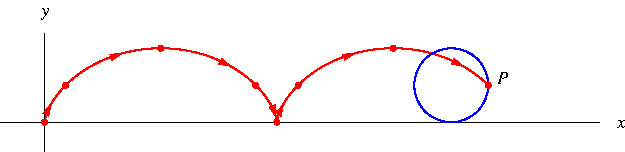
\includegraphics[width=12cm]{parametric-curves/pictures/11-01-cycloidh.pdf}%
%}%
%\only<handout:0| 9>{%
%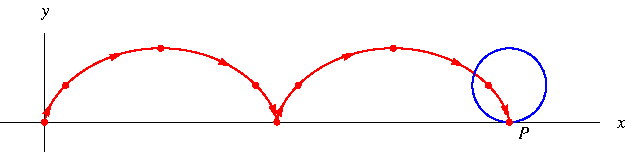
\includegraphics[width=12cm]{parametric-curves/pictures/11-01-cycloidi.pdf}%
%}%
%\only<handout:0| 10->{%
%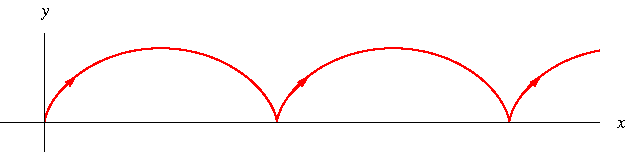
\includegraphics[width=12cm]{parametric-curves/pictures/11-01-cycloidj.pdf}%
%}%

\end{frame}
% end module cycloid-def
